\documentclass[11pt]{beamer}
\usetheme{Warsaw}
\usepackage[utf8]{inputenc}
\usepackage[brazil]{babel}  % idioma
\usepackage{amsmath,amsfonts,amssymb,textcomp}
\usepackage{graphicx}
\usepackage{subfigure}

\usepackage[lined]{algorithm2e}

% Configurando layout para mostrar codigos C++
\usepackage{listings}
%\usepackage{minted}
%pdflatex -shell-escape minted01.tex
%ou
%latexmk -pdf -shell-escape minted01.tex

\author{Othon Oliveira}
\title{Sistemas Operacionais}
%\setbeamercovered{transparent} 
%\setbeamertemplate{navigation symbols}{} 
%\logo{} 
\institute{Fatec -- Faculdade de Informática --- PE} 
%\date{} 
%\subject{} 
\begin{document}


% Capa - requer o TikZ
\newcommand{\capa}{
    \begin{tikzpicture}[remember picture,overlay]
        \node at (current page.south west)
            {\begin{tikzpicture}[remember picture, overlay]
                \fill[shading=radial,top color=orange,bottom color=orange,middle color=yellow] (0,0) rectangle (\paperwidth,\paperheight);
            \end{tikzpicture}
          };
    \end{tikzpicture}
}




\begin{frame}
\titlepage
\end{frame}

\begin{frame}
\tableofcontents
\end{frame}

%+++++++++++++++++++++++++++++++++++++++++++++++
\begin{frame}{Monitores -- Starvation}
\begin{figure}[h]
%\left

\includegraphics[width=18mm, height=15mm]{Figuras/appleOficial.jpg}
\qquad \quad \quad \quad \quad

\includegraphics[width=19mm, height=17mm]{Figuras/windows.png}
\qquad \quad \quad \quad \quad \quad \quad 	\vspace{1.0in}

\includegraphics[width=15mm, height=15mm]{Figuras/android.jpg}
\qquad \quad \quad \quad \quad \quad \quad \quad 

\includegraphics[width=25mm, height=15mm]{Figuras/ubuntu_904.jpg}

\end{figure}
\end{frame}


%+++++++++++++++++++++++++++++++++++++++++++++++
\section{ Deadlocks}
\subsection*{ Introdução aos Deadlocks}

\begin{frame}\frametitle{ Computadores e seus Recursos}
  
\pause
\begin{block}{ Recursos}
  Os computadores têm inúmeros recursos adequados para uso de um processo por vez, 
  podemos destacar a impressora, unidades de fitas (backup), entrada e saída nas tabelas do sistema.
\end{block}
 
 \pause
\begin{alertblock}{ Impasse}
 Se dois processos quiserem escrever simultaneamente na mesma impressora haverá um impasse. 
\end{alertblock}
 
\end{frame}


%--------------------------------------------------------
\begin{frame}\frametitle{ Um ou muitos recursos ??}

\begin{block}{ Acesso a muitos recursos}
  Para muitas aplicações, um processo necessita acesso exclusivo não somente a um recurso, mas também a vários
\end{block}

\pause
\begin{exampleblock}{ Mais de um recurso para um mesmo processo}
  O processo A solicita primeiro permissão para usar o Scanner e é autorizado.
  O processo B, que é programado diferentemente, solicita primeiro permissão para usar o gravador de CD e também é autorizado.
  Então o processo A pede para usar o gravador de CD, mas a solicitação é negada até que o processo B o libere. 
  Infelizmente, em vez de liberar o gravador de CD, o processo B pede para usar o Scanner, nesse ponto ambos os processos ficarão bloqueados 
  para sempre, isso é Deadlock. Isso também pode ocorrer com computadores numa rede ?
\end{exampleblock}

\end{frame}


%--------------------------------------------------------
\begin{frame}\frametitle{ Deadlocks em Banco de Dados}

\begin{exampleblock}{ Exemplo: dois processos querem fazer \textit{inserts} }
  Em sistemas de BD, um programa pode ter de bloquear o acesso a diversos registros quando estiver usando, a fim de evitar condições de disputa 
  (race condition). Se o processo A bloquear o acesso ao registro R1, o processo B bloquear o acesso ao registro R2 e depois cada processo tentar 
  bloquear o acesso ao registro do outro, teremos também um deadlock.
\end{exampleblock}

\pause
\begin{alertblock}{ Hardware e Software}
  Assim, deadlocks podem ocorrer tanto em recursos de hardeare com de softare.
\end{alertblock}
\end{frame}


%+++++++++++++++++++++++++++++++++++++++++++++++
\subsection*{ Recursos preemptíveis e não preemptíveis}

\begin{frame}\frametitle{ Retirar recursos ou não ?}

\begin{block}{ Recursos preemptível}
 Um recurso preemptível é aquele que pode ser retirado do processo proprietário sem nenhum prejuízo.
\end{block}

\pause
\begin{exampleblock}{ Memórias}
  A memória é um exemplo de recurso preemptível. O processo A necessita de 32 MB de memória e é lhe cedida, o processo B quer 32 MB 
  para imprimir algo. 
  O computador só tem disponível 32 MB num determinado momento, a qual dos dois recursos será negada/retirada o acesso aos 32 MB ?
\end{exampleblock}

\end{frame}


%------------------------------------------------
\begin{frame}{ Sequência de recursos}

\begin{alertblock} { Como usar recursos}
\begin{enumerate}
\pause
 \item Requisitar o recurso
\pause
 \item Usar o recurso
\pause
 \item Liberar o recurso
\end{enumerate}

\end{alertblock}
\pause
 Se o recurso não estiver liberado, quando requisitado, o processo será bloqueado.
\end{frame}


%------------------------------------------------------------

\begin{frame}{ Aquisição de recurso}
 \begin{block} { Para alguns tipos de processo}

\pause
  Para processos de usuários cabe a eles mesmos gerir o uso de recursos\\
\pause
  Uma maneira de permitir o usuário gerir recursos é associar um semáforo a cada recurso.\\
\pause
  Esses semáforos são todos inicializados com 1

 \end{block}
\end{frame}


%------------------------------------------------------------------
\defverbatim[colored]\lstDsp{
\begin{lstlisting}[language=Pascal,basicstyle=\ttfamily\small,keywordstyle=\color{blue},stringstyle=\color{verde},commentstyle=\color{red}, 
  extendedchars=true,showspaces=false,showstringspaces=false,numbers=left,numberstyle=\tiny,breaklines=true,backgroundcolor=\color{green!10},
  breakautoindent=true,captionpos=b,xleftmargin=0pt]

  typedef int semaforo;
  semaforo recurso_1;
  
  void processo_A(void){
    down(&recurso_1);
    use_recurso_1();
    libere(&recurso_1);
  }
\end{lstlisting}
}

\begin{frame}{ Requisitando recurso}{pseudo -- C}

  \lstDsp

\pause
\begin{exampleblock}{1 semáforo para 1 recurso}
  Uso de um semáforo para proteger um (1) recurso
\end{exampleblock}

\end{frame}

%------------------------------------------------------------------
\defverbatim[colored]\lstDsp{
\begin{lstlisting}[language=Pascal,basicstyle=\ttfamily\small,keywordstyle=\color{blue},stringstyle=\color{verde},commentstyle=\color{red}, 
  extendedchars=true,showspaces=false,showstringspaces=false,numbers=left,numberstyle=\tiny,breaklines=true,backgroundcolor=\color{green!10},
  breakautoindent=true,captionpos=b,xleftmargin=0pt]

  typedef int semaforo;
  semaforo recurso_1;
  semaforo recurso_2;
  
  void processo_A(void){
    down(&recurso_1);
    down(&recurso_2);
    use_todos_recurso_1();
    libere(&recurso_2);
    libere(&recurso_1);
  }

\end{lstlisting}
}

\begin{frame}{ Requisitando recursos}{pseudo -- C}

  \lstDsp

\pause

\begin{exampleblock}{semáforo para 2 recursos}
  Uso de um semáforo para proteger dois (2) recursos
\end{exampleblock}
\end{frame}

%------------------------------------------------------------------
\defverbatim[colored]\lstDsp{
\begin{lstlisting}[language=Pascal,basicstyle=\ttfamily\small,keywordstyle=\color{blue},stringstyle=\color{verde},commentstyle=\color{red}, 
  extendedchars=true,showspaces=false,showstringspaces=false,numbers=left,numberstyle=\tiny,breaklines=true,backgroundcolor=\color{green!10},
  breakautoindent=true,captionpos=b,xleftmargin=0pt]
  typedef int semaforo;
  semaforo recurso_1;
  semaforo recurso_2;
  
  void processo_A(void){
    down(&recurso_1);
    down(&recurso_2);
    use_todos_recurso();
    libere(&recurso_2);
    libere(&recurso_1);
  }
  void processo_B(void){
    down(&recurso_1);
    down(&recurso_2);
    use_todos_recurso();
    libere(&recurso_2);
    libere(&recurso_1);
  }

\end{lstlisting}
}
\begin{frame}{ Requisitando recursos}{ pseudo -- C}

  \lstDsp

\pause

\begin{exampleblock}{2 semáforo para 2 recursos}
  Uso de um semáforo para proteger dois (2) recursos
\end{exampleblock}
\end{frame}


%------------------------------------------------------------------------
\defverbatim[colored]\lstDsp{
\begin{lstlisting}[language=Pascal,basicstyle=\ttfamily\small,keywordstyle=\color{blue},stringstyle=\color{verde},commentstyle=\color{red}, 
  extendedchars=true,showspaces=false,showstringspaces=false,numbers=left,numberstyle=\tiny,breaklines=true,backgroundcolor=\color{green!10},
  breakautoindent=true,captionpos=b,xleftmargin=0pt]
  typedef int semaforo;
  semaforo recurso_1;
  semaforo recurso_2;
  
  void processo_A(void){
    down(&recurso_1);
    down(&recurso_2);
    use_todos_recurso();
    libere(&recurso_2);
    libere(&recurso_1);
  }
  void processo_B(void){
    down(&recurso_2);
    down(&recurso_1);
    use_todos_recurso();
    libere(&recurso_1);
    libere(&recurso_2);
  }

\end{lstlisting}
}

\begin{frame}{ Qual dos dois códigos está certo}{ O anterior ou este ?}

\lstDsp

\pause

\begin{exampleblock}{2 semáforo para 2 recursos}
  De acordo com os exemplos acima para proteger dois (2) recursos qual está certo?
\end{exampleblock} 

\end{frame}


%+++++++++++++++++++++++++++++++++++++++++++++++
\section{ Starvation}
\subsection*{ Introdução ao Starvation}


\begin{frame}\frametitle{ Starvation }

\begin{block}{ O que é Starvation?}
 Um processo com pouca prioridade pode ser que nunca seja selecionado
\end{block}

\pause
\begin{exampleblock}{ Situação}
  Em programação concorrente um processo ``morre'' de ``inanição'' quando nunca é selecionado porque outros processos com maior prioridade o 
  impedem de ser executado.
  \pause
  Caso os processos rodem indefinidamente pode ocorrer ``inanição'', contudo com fatias de tempo para cada processo isso pode ser resolvido?

\end{exampleblock}

\end{frame}

%----------------------------------------------------

\begin{frame}\frametitle{ Starvation ou inanição ?}

\begin{block}{ Fatia de tempo infinita}
 Caso um processo não tenha definição da fatia de tempo do processador, pode ocorrer que um processo com pouca prioridade nunca seja selecionado 
 pelo escalonador para ser executado
\end{block}

\pause
\begin{exampleblock}{ O jantar dos filósofos}
  \begin{itemize}
   \item Há cinco filósofos ao redor de uma mesa
   \pause
   \item Um garfo é colocado entre cada filósofo
   \pause
   \item O espaguete está escorregadio, o filósofo precisa de dois garfos para comer
   \pause
   \item Após comer o filósofo deve liberar o garfo que utilizou.
  \end{itemize}

\end{exampleblock}

\end{frame}

%+++++++++++++++++++++++++++++++++++++++++++++++
\begin{frame}{ O jantar de filósofos}
\begin{figure}[h]

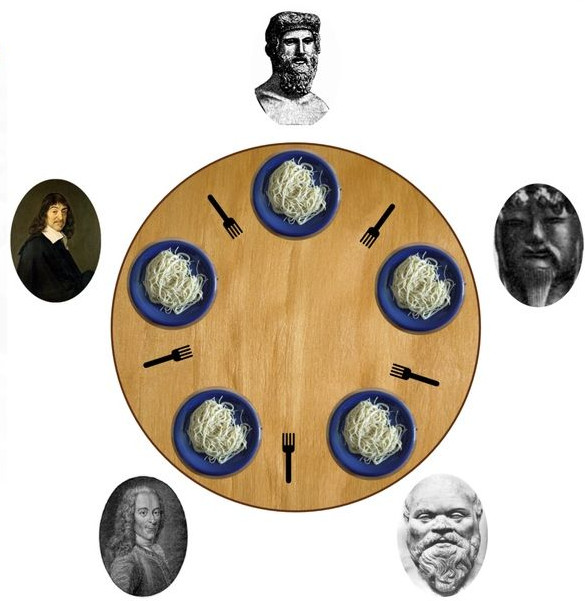
\includegraphics[width=100mm, height=60mm]{Figuras/filosofos.jpg}\\
\pause
Qual a melhor solução para não ocorre Starvation ?

\end{figure}


\end{frame}



\end{document}